\chapter{LITERATURE REVIEW}
\label{ch:litreview}

\section{Introduction}
This is a \LaTeX{} book~\parencite{basaran22}. \textcite{abdulrahman22} wrote a good~\LaTeX{} book. \textcite{edlom21} claimed that \\
According to \parencite{haynes18}, social media plays a significant role in the careers of independent musicians.
\textcite{hsu18} has three or more authors.
\textcite{shanmugam19} has three or more authors.
Two authors \parencite{igwenagu16}.
\textcite{jarvekulg21} has two authors.
Cite more than one article \parencite{kaur15,lee20}.
Cite more than one article \parencite{wambua23,wen21}.
Newspaper \parencite{leger21}.
\parencite{liang22}

\section{Local Musicians}
Local musicians are highly regarded in any community. These unsung music heroes perform in local hotels, tiny venues, and community events, sharing their love of music with their communities. These outstanding musicians lend a unique flavor to the local music industry by delivering a variety of styles and genres to suit their audience. Local musicians are storytellers who express their community's experiences, traditions, and emotions via their music. They become part of the local culture since their performances unite the audience. \\

According to \textcite{mohd21}, Local musicians in Malaysia play a crucial role in maintaining and promoting Malaysia's unique musical heritage. Malaysia's local singers serve as cultural ambassadors, representing the country's rich culture through the genres of Malay, Chinese, Indian, and indigenous music. They showcase the historical development of distinct Malaysian musical styles \parencite{mohd21}. By blending both traditional and modern sounds, they construct an evolving musical world that deeply connects with enthusiasts of music, establishing an inclusive identity where venues and events act as main places for gathering \parencite{ong19}. Malaysian musicians incorporate international musical trends while showcasing the nation's diverse heritage, encompassing traditional gamelan music to contemporary urban hip-hop. They perform at festivals, night markets, and cultural events, fostering solidarity among individuals from various origins through the unifying power of music in this global community. 

\subsection{Local Music Scene Trends}
\textcite{ong19} has observed that the local music scene in Malaysia has undergone substantial development in recent years, particularly in Kuala Lumpur, where a vibrant Indie Rock music community has emerged. This community prioritizes online connection and collaboration with the international and regional music scenes, promoting the development of independent labels that endorse regional Indie music. These labels offer a forum for musicians to produce music that departs from the worldwide popularised local rock and pop music genres. However, there are ongoing difficulties, mainly due to a lack of suitable locations for Indie Rock music performances. This issue has been further aggravated by the closing of major venues, resulting in a significant impact on the local Indie Rock music scene. Despite these obstacles, the community displays persistence by actively pursuing additional performing spaces and events that increase musical exposure and promote the development and endurance of local Indie Rock performers. \\

In addition, as emphasized by \textcite{mohd21}, the music industry in Malaysia has seen an engaging pattern of blending traditional Malaysian musical components with contemporary genres, resulting in a unique and varied musical environment. This fusion has not only gained popularity in Malaysia but has also attracted international acclaim, hence enhancing the global prominence of Malaysian music. Moreover, there is an emerging pattern of Malaysian artists engaging in partnerships with musicians from other countries, leading to the exchange of cultural elements and the integration of many musical influences into the domestic music landscape. This instance highlights the adaptability and creativity of Malaysian musicians in connecting different cultures through their music. \\

Furthermore, \textcite{silahudin19} has seen an increasing popularity of indie and alternative music genres in Malaysia, with local and worldwide acclaim being achieved by independent musicians and bands. This phenomenon has played a significant role in fostering a dynamic and varied music scene within the nation. In addition, Malaysian musicians have been engaging in the exploration of traditional sounds, combining them with modern elements to produce unique and different musical expressions. The expansion of digital platforms and social media has additionally furnished Malaysian musicians with fresh opportunities to exhibit their work, establish connections with listeners, and participate in partnerships with artists from various countries, leading to a more interconnected and globalized music scene in Malaysia. These trends collectively demonstrate the ever-changing and progressive nature of Malaysia's local music landscape.

\subsection{Local Music Scene Challenges}
The local music scene in Malaysia encounters substantial obstacles, mostly due to the lack of performance venues for Indie Rock music \parencite{ong19}. The closing of major venues has hurt the visibility of the local Indie Rock music scene, underscoring the urgent requirement for additional performance spaces and concerts that promote the development and longevity of local Indie Rock musicians. The limited number of available venues has presented challenges for musicians and organizers, limiting the growth and visibility of Indie Rock music in the local music scene. \\

In addition, as highlighted by \textcite{mohd21}, the music industry in Malaysia has numerous challenges. A notable obstacle comes in the attempt of local artists to acquire exposure and recognition in the highly competitive industry. The lack of resources and opportunities for independent musicians, coupled with the growing popularity of mainstream commercial music, present significant challenges to the development of the local music scene. Moreover, the problems associated with music piracy and copyright infringement have significantly affected the financial well-being of musicians and the long-term survival of the music industry in Malaysia. These challenges emphasize the necessity for increased assistance and infrastructure for the development and promotion of talents within the local music scene. \\

Furthermore, the music industry in Malaysia encounters specific challenges. An important obstacle is the insufficient assistance and promotion available to native musicians, particularly those who produce music in native languages or dialects \parencite{silahudin19}. This presents an obstacle to the preservation and development of Malaysia's diverse musical legacy. Moreover, the growing popularity of popular commercial music and global music trends could surpass the importance of local talents, posing a challenge for up-and-coming Malaysian artists to establish themselves in the industry. Moreover, the pressing concerns of copyright protection, fair compensation, and sustainable income for artists in the digital age emphasize the necessity for improved rules and support structures to guarantee the livelihood of traditional music artists in Malaysia. The related challenges highlight the many barriers that the local music industry is currently encountering.

\subsection{Music Promotion Strategies}
\subsubsection{Digital Marketing}
Music promotion has experienced an important shift in the current era of technology, with digital marketing emerging as a crucial element for both musicians and record companies. The proper utilization of online platforms can determine an artist's success in the fiercely competitive music industry. According to \textcite{haynes18}, social media enables direct interaction with the audience, which is a crucial aspect of promoting digital music. Nevertheless, their research also underscores the limitations of social media in accessing new audiences. \\

Digital marketing involves using several platforms to effectively target a wide demographic. Social media networks like Instagram, Facebook, and Twitter have a crucial impact. Artists and labels ought to consistently keep dynamic profiles, interact with fans, and regularly release captivating stuff. Musicians utilize social media channels to communicate with their audience, yet these platforms may have limitations in terms of reaching new audiences \parencite{haynes18}. This emphasizes the significance of expanding promotional techniques. \\

Developing and distributing captivating content is essential in the promotion of digital music. In addition to releasing music, artists can give exclusive insights into their creative process, music videos, and live performances. Employing visual media like YouTube and TikTok can also produce favorable outcomes. \textcite{basaran22} highlight the importance of customizing digital material and its influence on consumer happiness in the era of digital entertainment. In addition, they analyze the impact of social media on digital marketing, highlighting the fact that having a strong online presence does not always result in financial success for musicians. \\

Effective music promotion in the current digital context heavily relies on the implementation of digital marketing methods. To advance their music career, artists and labels should utilize social media, email marketing, and other content forms to engage with their audience, expand their influence, and eventually propel their music careers. By adopting these strategies and acknowledging their limitations, musicians can distinguish themselves in a saturated market and develop a loyal following, as evidenced by the studies conducted by \textcite{haynes18,basaran22}.

\subsubsection{Fan Engagement}
Interactive creation of content is a highly successful method for engaging fans. This includes live streaming sessions, question and answer sessions, and exclusive insights into the artist's personal life. This type of content cultivates a feeling of closeness and relationship between the artist and the fans. \textcite{edlom21} argue that fans actively participate in the creation of value within music brand communities by establishing emotional bonds and aligning their values with those of the artists. \textcite{lee20} explore participatory fandom, which emphasizes the active role of fans in shaping music promotion and exercising influence on commercial music services. \\

Personalization plays a crucial role in promoting fan involvement. Artists and labels can utilize email marketing and social media platforms to establish direct communication with their fans. This allows them to personalize the content by addressing fans by their names and personalizing it to their interests. Delivering customized messages for important occasions such as birthdays or album celebrations, expresses gratitude and strengthens the bond between the artist and their fans. Customized communication creates a sense of appreciation among followers and motivates them to maintain their loyalty and support. This is consistent with the dynamics of fan networks and their interactions with artists in a digital context, as explored by \textcite{edlom21}. \\

Establishing a digital community focused on the artist's music is an effective approach to engage fans. Artists can establish fan clubs, forums, or exclusive groups on popular platforms such as Facebook or Discord. These spaces provide opportunities for fans to interact, express their enthusiasm for the music, and participate in conversations. The artist's active engagement in these groups develops a feeling of belonging and guarantees that fans receive sufficient details about upcoming releases and activities. \textcite{lee20} found that the connection between music enthusiasts and commercial music platforms is shaped by participatory fandom, highlighting the significance of fan involvement in music promotion. \\

Fan engagement is more than an aspect of music promotion; rather, it serves as the core foundation upon which successful music careers are established. Strategies such as creating interactive material, engaging in personalized contact, and promoting a sense of community are crucial for establishing deep connections with followers. Both \textcite{edlom21} and \textcite{lee20} emphasize that these connections can result in increased audience pleasure, collaborative value creation, and sustained support for the artist's work. By placing audience involvement as a top priority, musicians and record labels can establish a durable and successful music ecosystem in the digital age.

\section{Online Community}
An online community is described as a digital space where individuals who have similar interests, objectives, or affiliations gather to communicate, share information, and participate in discussions or activities. Communities may exist in diverse formats, including forums, social media groups, or specialized platforms, offering members a virtual space to communicate, cooperate, and develop connections without being constrained by geographical limitations. Online community platforms such as Facebook Groups, Reddit, LinkedIn Groups, Discord servers, and niche-specific forums like Stack Overflow for programming enthusiasts or GitHub for software developers serve as examples. These platforms enable the establishment of communities centered around diverse subjects, spanning from personal interests and professional connections to mutual aid organizations and enthusiast associations.

\subsection{User-Generated Content}
According to \textcite{v22}, User-Generated Content (UGC) in online communities offers a diverse range of values, including functional, emotional, and social components. Functionally, user-generated content (UGC) frequently functions as a valuable source of information, guidance, and resolutions for members of a community. Emotionally, it cultivates a feeling of inclusion and mutual experiences, fostering emotional bonds among users. From a social perspective, user-generated content (UGC) plays a significant role in encouraging the development of a unified community, where individuals join based on common interests or objectives. This multidimensional value enhances participation and connection among community members. \\

The trust-building influence of user-generated content (UGC) in digital media, which is favored above traditional advertising \parencite{v22}. UGC is characterized by its authenticity, making it widely regarded as more genuine and reliable compared to content produced by professionals. Online communities place high importance on the thoughts and experiences given by their members, acknowledging them as genuine and trustworthy sources. The confidence and authority that is built through User-Generated Content (UGC) significantly impact the dynamics of a community and the level of influence its members have. \\

The quality of user-generated content (UGC) in online communities is impacted by multiple factors, as outlined by \textcite{luca21}. These elements include promotional content, peer effects, biases, and self-selection. UGC of superior quality frequently arises when individuals are driven by non-monetary incentives, such as badges or social standing, to provide excellent content to the community. These incentives can guide user contributions in a good manner, promoting the development of significant and influential content \parencite{luca21}. Hence, the interaction between the standard of content and the motivating factors has an important effect on the structure of user-generated content inside digital media platforms.\\

\begin{figure}[h]
    \centering
    
\includegraphics[width=0.9\linewidth]{mainmatter/images/ugc1.png}
    \caption{User-Generated Content (UGC) in TikTok}
    \caption*{TikTok post by @josephro53 (2021, June 22) [ByteDance, 2023]}
    \label{fig:myfig1}
\end{figure}
Within the realm of user-generated material in online communities, it is useful to analyze two illustrative examples that demonstrate its influence and variety. The first figure involves a TikTok video review conducted by user @josephro53, which explores the realm of those who hold a deep passion and knowledge about sneakers. This user-generated material has a reviewer who offers a perceptive and subjective evaluation of the Makerz Rentaka sneakers. This content provides analytic value to viewers seeking product knowledge and a sense of connection with fellow sneaker enthusiasts who share a passion for the topic. \\

\begin{figure}[h]
    \centering
    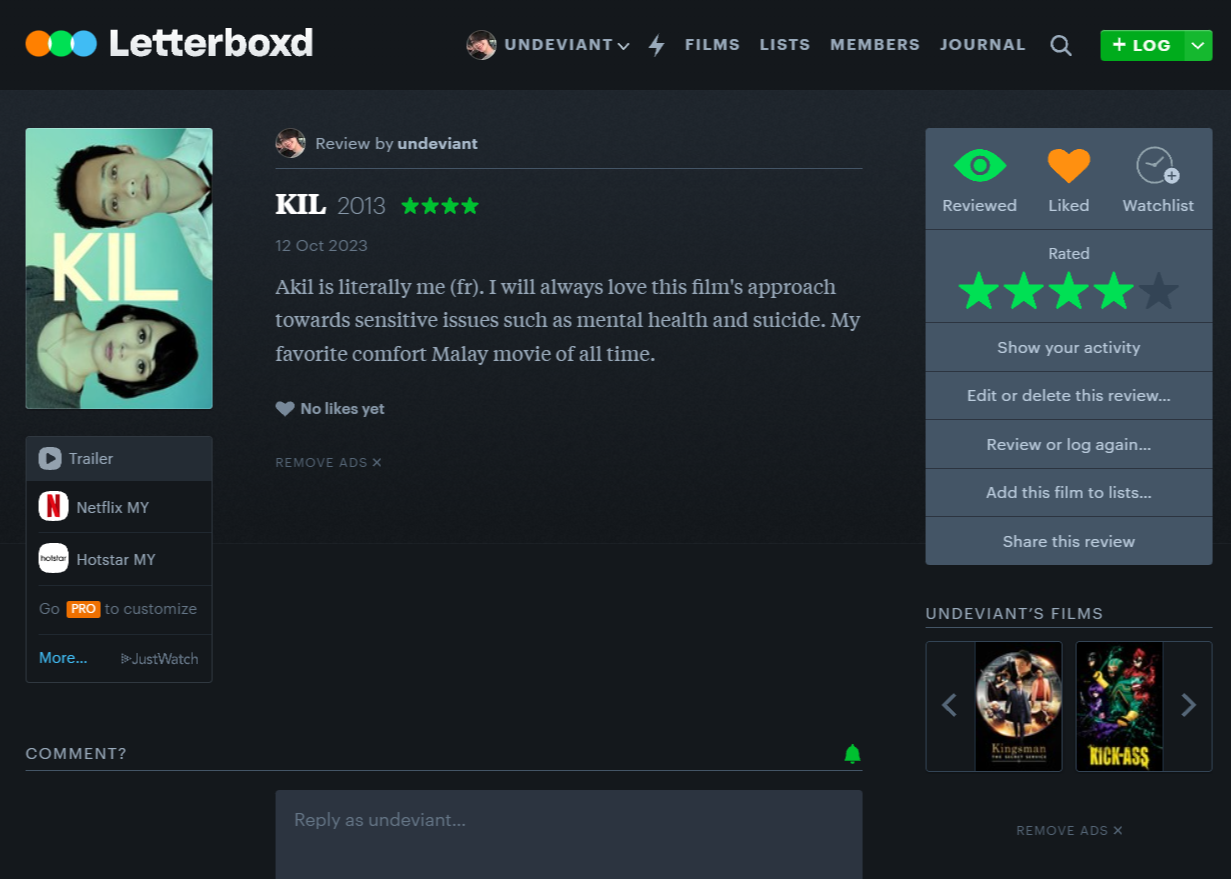
\includegraphics[width=0.8\linewidth]{mainmatter/images/ugc2.png}
    \caption{User-Generated Content (UGC) in Letterboxd}
    \caption*{Letterboxd post by @undeviant (2023, October 12) [Letterboxd, 2023]}
    \label{fig:myfig2}
\end{figure}
The second figure, a movie review of "KIL (2013)" by user @undeviant on Letterboxd, illustrates the significance of user-generated content (UGC) in the area of cinema critique and admiration. In this review contributed by @undeviant, a perceptive evaluation of the Malaysian movie is presented, presenting an original viewpoint that enhances the discussion about the film. This material represents the trust and authority that users give to other community members when they are looking for recommendations or insights in their areas of interest.

\subsection{Social Media Integration}
The integration of social media into online communities has become an essential feature of modern digital interactions. This integration utilizes the capabilities of platforms such as Facebook, Twitter, and Instagram to improve the overall community experience. Online communities promote enhanced user involvement and exposure by enabling the seamless linking of social media profiles and content sharing. Integrating social media not only expands the audience for community content, but also promotes immediate conversations, exchange of valuable knowledge, and fast distribution of information \parencite{zanuar22}. This technology bridges the boundaries between virtual communities and the wider online social environment, allowing members to easily interact, cooperate, and contribute across several platforms, hence enhancing the overall community experience.

\subsection{Types of Interaction}
Interactions in online communities are complex and diverse, with different forms that each have their importance. Primarily, likes and reactions provide members with a convenient and efficient means to show their approval or appreciation for a post or comment. These confirming actions aim to inspire content authors and communicate that their efforts are highly esteemed in the community. Moreover, comments serve as the vital essence of discussions, offering a platform for individuals to express their opinions, pose inquiries, and participate in important conversations. Comment threads frequently develop into rich sources of knowledge, deep opinions, and varied points of view, promoting a feeling of community unity. \\

Sharing content is a crucial method for interaction within internet communities. When a member shares a post or discussion topic, it expands the visibility of that information to a wider audience, potentially recruiting new members and improving the overall reach of the community. Upvotes and downvotes, frequently observed on sites such as Reddit, allow users to indicate their approval or disapproval of particular posts or comments. This voting method helps the curation of content, guaranteeing that the most relevant and significant contributions rise to popularity, while irrelevant or improper content is dismissed. Furthermore, ratings and reviews have a crucial significance, particularly among communities that prioritize items, services, or information. Users can allocate ratings and submit comprehensive reviews, providing essential input and impacting the decisions of others. These assessments enhance knowledge and assist members in selecting the best services. \\

In addition to these interactions, mentions and tags play a crucial role in engaging particular community members in discussions and recognizing their expertise. Direct messaging enables confidential individual conversation, but polls and surveys provide a systematic approach to collecting community comments, opinions, or preferences. Emojis and reaction buttons serve to enhance the expression of emotions and sentiments towards content, providing additional depth and subtlety. These various types of interaction collectively enhance the overall experience of online communities by promoting communication, collaboration, and engagement among members, hence increasing their appeal and effectiveness as platforms. \\

When discussing online communities, it is essential to acknowledge the influence of incorporating social media on the dynamics of the community and the level of involvement from its members. \textcite{zanuar22} highlight the effectiveness of social media tactics for independent artists. These tactics encompass actively interacting with supporters, revealing exclusive content, and maintaining genuineness and consistency in social media posts. Through the incorporation of social media platforms into their digital communities, independent artists can establish direct connections with their audience, providing exclusive perspectives into their creative approaches, and developing a loyal following that actively engages in conversations and promotional activities. \\

In addition, \textcite{jarvekulg21} discusses the differences between brand-centric and community-focused strategies for promoting music on social media. The difference is important in the context of online communities, as it indicates the different ways through which community members and artists interact with each other. The brand-centered method prioritizes promotional gatekeeping and conventional marketing techniques, whereas the community-oriented approach places importance on establishing significant ties with fans and fellow artists. By incorporating these methods into online communities, a comprehensive music promotion plan may be developed that addresses both user involvement and brand establishment, resulting in a well-rounded experience for community participants. In short, the incorporation of social media into online communities acts as a connection between artists and their audience, encouraging interaction, genuineness, and a variety of promotional approaches.

\subsubsection{Gamification Elements}
Introducing gamification features into an online community can significantly influence its dynamics and enhance member participation. Gamification, as defined by \textcite{hsu18}, refers to the utilization of game components in non-game situations to modify individuals' behavior and enhance their level of involvement. This concept has attracted significant attention in several fields, such as online communities, where it can play a crucial role in improving the overall user experience. \\

An essential aspect commonly employed in online communities to enhance user engagement is the incorporation of points, badges, and levels. According to \textcite{mauroner19}, these elements can be effective strategies for identifying and inspiring community members. Points and badges provide individuals with a feeling of accomplishment and status, motivating them to actively engage and demonstrate their expertise. Through the process of measuring their contributions and evaluating them based on leaderboards, individuals are motivated to consistently enhance and make valuable additions to the community's discussions and activities. \\

Furthermore, the incorporation of technical challenges and quests in the community is consistent with the user engagement concepts emphasized by \textcite{hsu18}. These challenges offer an exhilarating opportunity for cooperative learning and problem-solving. These activities enhance the problem-solving abilities of participants and promote a feeling of togetherness as they collaborate to overcome obstacles. \\

In addition, the introduction of virtual currencies and rewards can significantly influence the dynamics of an online community. These elements can be utilized to encourage participation and reward members for their contributions \parencite{mauroner19}. Virtual currencies can be used to purchase virtual goods, which can be utilized to enhance the user experience. These elements can be used to encourage participation and reward members for their contributions. Virtual currencies can be used to purchase virtual goods, which can be utilized to enhance the user experience. \\

\begin{figure}[h]
    \centering
    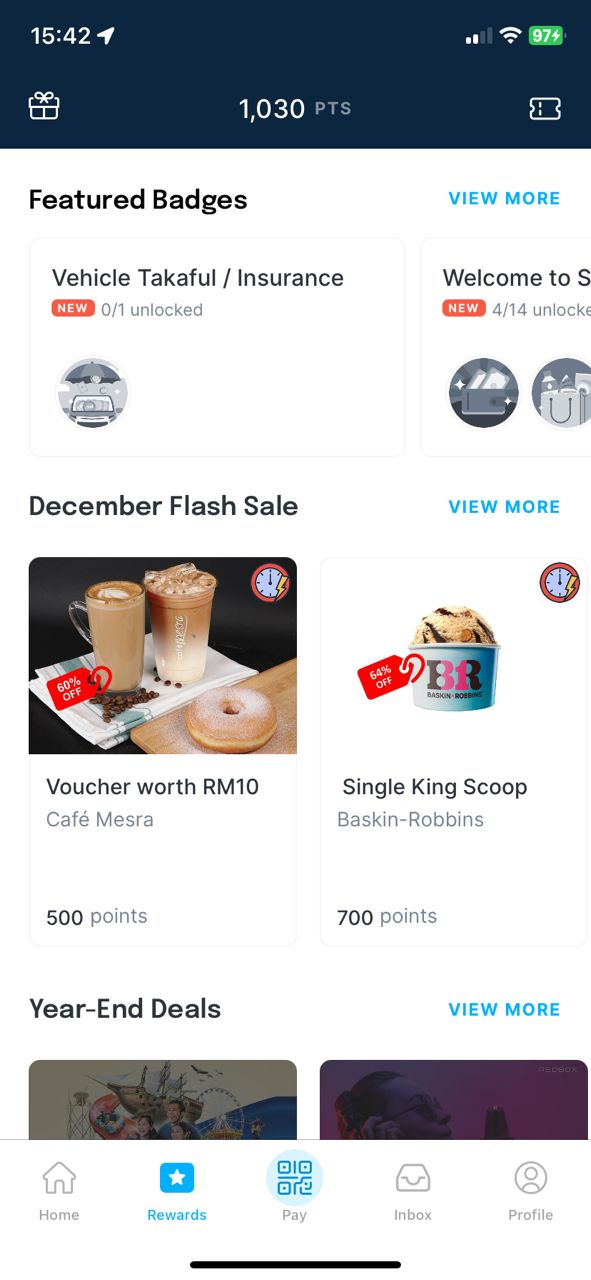
\includegraphics[width=0.35\linewidth]{mainmatter/images/gami1.jpg}
    \caption{Gamification Elements in Setel}
    \caption*{Screenshot of Rewards page in Setel (2023, December 30) [Setel Ventures Sdn. Bhd., 2023]}
    \label{fig:myfig3}
\end{figure}
Figure 2.3 illustrates the gamified rewards page of the Setel mobile application, which is a comprehensive platform designed for the Malaysian audience, offering services such as fuel, parking, EV charging, eWallet, and more. This page utilizes gamification to prominently display users' earned points, promoting engagement by transforming routine transactions into chances to earn rewards. Users are motivated to actively engage in Setel's products, earning points that can be redeemed for practical vouchers in various categories such as food, fashion, and entertainment. The implementation of gamified design in Malaysia aims to provide an engaging and captivating experience for users. By using the principles of incentive and achievement, this design strategy fosters user loyalty. Additionally, it offers real and appealing rewards to further enhance user engagement.

\section{Music Discovery}

\subsection{Music Genre Diversity}
The concept of an extensive variety of genres in the process of discovering music has seen significant growth throughout recent years, driven by user-focused observations and developments in recommender systems. \textcite{robinson20} clarify the complex and varied aspects of diversity in music recommendation lists, underscoring the significance of integrating both internal and external diversity. Internal diversity, in this context, pertains to the assortment of subgenres and styles within a specific genre, whereas external diversity incorporates recommendations from entirely separate genres. These subtle and precise categories have fundamentally changed the way music enthusiasts explore and value varied musical landscapes. \\

In current recommender systems, measures such as variety, creativity, and randomness have become essential in addition to accuracy. When utilized in music discovery systems, these measures have a crucial impact in promoting genre exploration and expanding listeners' musical horizons. Diversity, as per the definition provided by \textcite{robinson20}, extends beyond the mere inclusion of random music. It encompasses the goal of achieving a well-proportioned representation of various genres and subgenres within recommendation lists. The presence of variety in music drives users to explore unfamiliar and unexplored musical categories, while randomness adds an element of pleasant unexpectedness, allowing listeners to come across genres they may not have encountered otherwise. \\

By utilizing user-centric information and metrics, modern music discovery services employ algorithms and curated playlists to direct listeners toward a wider range of genres. Through the integration of diverse elements from both internal and external sources, these platforms provide customized experiences that surpass the limitations of specific genres, promoting a wider and fulfilling musical exploration for users. Despite this changing environment, the recognition and enjoyment of many musical genres not only demonstrate the progress of technology but also highlight the influence of recommender systems in creatively influencing our musical preferences and tastes.

\subsubsection{Underrepresented Genres}
Traditional and local pop music, which is strongly influenced by tradition, frequently encounter difficulties in establishing a presence within popular music that appeals to a wider audience. However, online platforms have created an opportunity for enthusiasts to interact, exchange, and celebrate these genres. Online communities have arisen, attracting enthusiasts and musicians who are passionate about preserving and developing traditional music genres. Within these digital platforms, traditional and regional pop music genres receive acknowledgment and active involvement from an avid group of enthusiasts. \\

Digital platforms have a larger impact that goes beyond the establishment of genres. They facilitate the creation of music communities, surpassing geographical limitations and enabling persons with similar interests to unite. According to \textcite{silahudin19}, social media and online forums offer an environment for conversations, music sharing, and cooperation between musicians and their supporters. These groups not only cultivate admiration for underrepresented genres but also promote the production of novel music that combines traditional aspects with modern influences. \\

Eventually, the less popular music genres in the Malaysian music industry are discovering their expression and following the impact of digital platforms and online communities, as highlighted by \textcite{silahudin19}. These platforms facilitate the creation of genres such as traditional and regional pop music and promote the development of enthusiastic music communities. Thus, the music scene in Malaysia has grown in variety and comprehensive, preserving traditional practices while embracing originality and experimentation.

\subsection{Music Streaming Services Platforms}
Within the era of streaming, the process of discovering music has evolved and been shaped by both subjective experiences and social divisions based on socioeconomic status. \textcite{ellis20} explores the concept of "phenomenological moment" in the context of music discovery. He highlights the significant role these moments play in influencing individuals' interpretations and understandings of music. Music streaming platforms have emerged as a means of facilitating such experiences, allowing users to delve into a wide range of musical genres and artists that are customized to their preferences. These systems employ recommendation algorithms to enable users to find new music that connects with them, hence boosting the experiential aspects of music exploration. \\

In addition, users have progressively turned to music streaming sites as a method of storing and organizing their playlists \parencite{ellis20}. This method enables individuals to establish meaningful relationships with music over time, forming personal stories and connections with the songs they choose. Playlists surpass being simply collections of songs; they reflect an individual's musical journey and ever-changing preferences. This phenomenon highlights the fact that music streaming platforms not only make it easier to discover new music but also allow users to actively define their musical preferences and tastes. \\

\textcite{webster19} also explores the impact of music streaming platforms on individual preferences for music and the differentiation of cultural identities. These platforms have equalized access to music, erasing social class distinctions and enabling individuals from various backgrounds to explore and appreciate a wide variety of genres. Streaming services break common perceptions of modern and popular music by promoting user exploration free from the limitations of traditional class-based musical classifications. Music streaming platforms have played a significant role in creating a more inclusive and diversified music scene, prioritizing individual preferences over social class distinctions.

\subsubsection{Apple Music}

\subsubsection{Spotify}

\subsubsection{YouTube Music}

\subsection{User Preferences}

\section{Mobile Application}

\subsection{Type of Mobile Application}

\subsubsection{Native Application}

\subsubsection{Web Application}

\subsubsection{Hybrid Application}

\subsection{User Experience Design}

\subsection{Challenges of Mobile Application Development}

\subsection{Features of Mobile Application}

\subsubsection{Profile Creation}

\subsubsection{Music Snippet Sharing}

\subsubsection{Favourite/Bookmark}

\subsubsection{Ratings or Reviews}

\section{Reviews of Existing Mobile Application}

\subsection{Letterboxd}

\begin{itemize}[\label{}]
    \item \textbf{Advantages} \\
    test

    \item \textbf{Limitations} \\
    test
\end{itemize}

\subsection{Spotify}

\begin{itemize}[\label{}]
    \item \textbf{Advantages} \\
    test

    \item \textbf{Limitations} \\
    test
\end{itemize}

\subsection{Twitch}

\begin{itemize}[\label{}]
    \item \textbf{Advantages} \\
    test

    \item \textbf{Limitations} \\
    test
\end{itemize}

\subsection{Bandcamp}

\begin{itemize}[\label{}]
    \item \textbf{Advantages} \\
    test

    \item \textbf{Limitations} \\
    test
\end{itemize}

\subsection{SoundCloud}

\begin{itemize}[\label{}]
    \item \textbf{Advantages} \\
    test

    \item \textbf{Limitations} \\
    test
\end{itemize}

\section{Chapter Summary}